% ===========================================================================
\section{Sensitivity Analysis}
\label{sec:sensitivity}

The equilibrium conclusions so far were computed for one utility
function and, in Section~\ref{sec:bayesian}, one author population.
This section varies both.

\subsection{The \texorpdfstring{\textup{\textsc{share}}}{SHARE} payoff}
\label{sec:sensitivity-share}

To assess robustness to the utility function, we normalize the
\textup{\textsc{take}} payoff to $1$ and vary the
\textup{\textsc{share}} payoff $\sigma \in (0, 1)$:
\begin{center}
\begin{tabular}{lcc}
  \toprule
  Decision & Dictator & Recipient \\
  \midrule
  \textup{\textsc{share}} & $\sigma$ & $\sigma$ \\
  \textup{\textsc{take}}  & $1$      & $0$ \\
  \bottomrule
\end{tabular}
\end{center}
The decision matrix $d_{ij}$ is fixed by the tournament; only the
payoff weights change.
This parameterization loses nothing: utilities are equivalent up to
positive affine transformation (shifts of $u$ shift every entry of
$A$ uniformly and cancel in the softmax; scale is absorbed into
$\beta$), so any utility function reduces to the pair
$\bigl(\sigma,\, \beta\, u(E)\bigr)$ with
$\sigma = u(E/2)/u(E)$ after normalizing $u(0) = 0$.
The constants of Section~\ref{sec:properties} become
$\delta = 1 - \sigma$, $g = \sigma$, and
$\rho = \sigma / (1 - \sigma)$.
Two consequences frame the sweep.
First, midpoint concavity gives $u(E/2) \ge u(E)/2$ for every concave
utility, so \emph{risk-averse preferences occupy only the upper half}
$\sigma \ge 1/2$ of the parameter range.
Second, logarithmic utility corresponds to
$\sigma = \ln(1 + E/2)/\ln(1 + E)$, which increases with the
endowment; $E = 60$ gives $\sigma = \ln 31 / \ln 61 \approx 0.835$,
and the matched precision for the $\beta = 20$ analysis of
Section~\ref{sec:results-softmax} is
$\beta' = 20 \ln 61 \approx 82$.

\begin{figure}[!t]
\centering
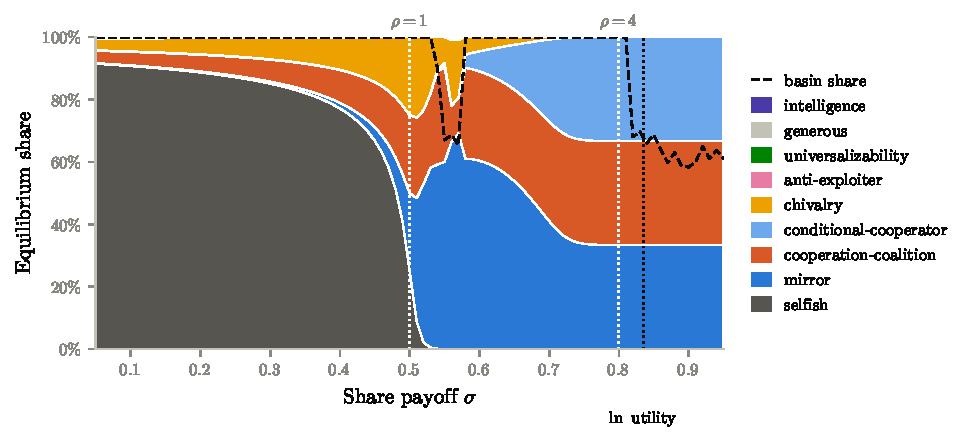
\includegraphics{share_sweep.pdf}
\caption{Softmax equilibrium as a function of the
\textup{\textsc{share}} payoff $\sigma$
(\textup{\textsc{take}} normalized to $1$), at precision matched to
the logarithmic-utility analysis ($\beta' = 20 \ln 61$).
The bands give the composition of the equilibrium reached from the
uniform prior; colors as in Figure~\ref{fig:trajectories}.
The dashed line is the fraction of $300$ random starts that reach
this equilibrium: where it falls below one, a rival basin exists.
Dotted verticals mark the exchange-rate thresholds $\rho = 1$
($\sigma = 0.5$), below which a share costs more than it delivers
and the field collapses to defection, and $\rho = 4$
($\sigma = 0.8$), above which the protection configuration becomes
self-sustaining; the mark at $\sigma = \ln 31/\ln 61 \approx 0.835$
is the game of the preceding sections.}
\label{fig:share-sweep}
\end{figure}

Figure~\ref{fig:share-sweep} traces the equilibrium reached from the
uniform prior across $\sigma \in [0.05, 0.95]$, together with the
share of random starts that reach it.
The sweep resolves into three regimes whose boundaries are exchange
rates.

\paragraph{Defection below $\rho = 1$.}
For $\sigma < 1/2$ a mutual \textup{\textsc{share}} ($2\sigma$) pays
less than a mutual \textup{\textsc{take}} ($1$): cooperation is a
net loss even when reciprocated.
The unique equilibrium concentrates on \textbf{Selfish} ($91\%$ of
the field at $\sigma = 0.05$), and the residual mass sits on the two
second-order enforcers --- the strategies that share most sparingly
against such a field.
By the concavity bound above, this regime is reachable only by
risk-seeking utility functions.

\paragraph{Cooperation above $\rho = 1$.}
At $\sigma = 1/2$ the cooperation surplus vanishes and the
equilibrium is a knife-edge four-way tie
(\textbf{Mirror}, \textbf{Cooperation coalition},
\textbf{Chivalry}, \textbf{Selfish} at $1/4$ each).
Beyond it, defection collapses abruptly --- \textbf{Selfish} holds
$9\%$ at $\sigma = 0.51$ and under $10^{-3}$ by $\sigma = 0.55$ ---
and a \textbf{Mirror}-led cooperative equilibrium takes over,
tightening to the enforcement core
(\textbf{Mirror}, \textbf{Cooperation coalition},
\textbf{Conditional cooperator} at one third each) by
$\sigma \approx 0.75$.
(A transitional second basin, \textbf{Mirror}-heavy with the two
enforcers, appears briefly for $\sigma \in [0.54, 0.57]$.)

\paragraph{Bistability above $\rho = 4$.}
The protection configuration of Section~\ref{sec:results-basins}
becomes an attractor only near the top of the range.
In the sharp limit the threshold is exact: at the five-member
protection point every member earns $2\sigma$ per encounter, while
the excluded \textbf{Cooperation coalition} earns
$(4 + 5\sigma)/5$ --- it harvests $\delta$ from four strategies but
loses the single share $g$ withheld by the protector --- so the
configuration repels its rival norm if and only if
$4\delta < g$, i.e.\ $\rho > 4$, i.e.\ $\sigma > 0.8$.
Empirically the second basin appears at $\sigma = 0.82$ and claims
$48\%$ of random starts by $\sigma = 0.95$.
Read back through the endowment, $\rho(E) > 4$ requires
$E > 25.6$ under logarithmic utility: the enforcement--protection
bistability of Section~\ref{sec:results-basins} is a
\emph{large-stakes} phenomenon.
For endowments below ${\approx}26$, enforcement is the only
attractor and \textbf{Chivalry}'s norm cannot sustain itself; as
$E \to \infty$, $\rho \to \infty$ and the pool moves ever deeper
into the bistable regime.

\subsection{The author-type composition}
\label{sec:sensitivity-types}

The results of Sections~\ref{sec:bayesian}
and~\ref{sec:bayesian-bloc} were computed for one author population
--- $0.4$ own-payoff, $0.4$ mixed ($\lambda = 0.5$), $0.2$
total-welfare.
To test how much hangs on that choice, we recompute the mixture
fixed point of Equation~\eqref{eq:mixture-fixed-point} over the full
simplex of type masses (step $0.1$, $\beta = 20$, multi-start),
sweep the mixed type's welfare weight $\lambda$ from $0$ to $1$ at
the reference masses, and rerun the bloc scan of
Section~\ref{sec:bayesian-bloc} at bloc masses from $0.05$ to
$0.5$.

\paragraph{The interior of the simplex is unanimous.}
For every composition with own-payoff mass between $0.2$ and $0.8$
--- whatever the split of the remainder between mixed and
total-welfare types --- multi-start sampling finds a \emph{single}
fixed point: the enforcement core
(\textbf{Mirror}, \textbf{Conditional cooperator},
\textbf{Cooperation coalition} at one third each), attaining the
first-best welfare.
The $\lambda$ sweep is equally flat: at the reference masses every
$\lambda \in [0, 1]$ yields that same unique fixed point.
The equilibrium in the bottom row of Figure~\ref{fig:trajectories}
is not a feature of the particular mixture we happened to choose;
it is the generic outcome for any substantially heterogeneous
author population.

\paragraph{Multiplicity survives only at the corners.}
Near the pure own-payoff corner the protection attractor of
Section~\ref{sec:results-basins} persists, but a small admixture of
welfare-weighing authors destroys it: about $11\%$ total-welfare
mass suffices, or about $20\%$ mixed mass at $\lambda = 0.5$ ---
in both cases an \emph{effective welfare weight}
$\sum_t m_t \lambda_t \approx 0.1$.
The enforcement--protection bistability is a monoculture
phenomenon: objective heterogeneity acts as an equilibrium-selection
device, and it selects enforcement.
At the opposite corner, with no own-payoff mass at all, equilibria
multiply for the opposite reason.
Welfare-maximizing authors are indifferent among welfare-tied
configurations, and the fixed points are five-member full-cooperation
supports at one fifth each (for instance \textbf{Mirror},
\textbf{Anti-exploiter}, \textbf{Universalizability},
\textbf{Chivalry}, \textbf{Generous} --- or the variant with
\textbf{Conditional cooperator} and \textbf{Intelligence} in place
of the last two) with welfare identical to four decimal places; the
prior selects among them.
Welfare is pinned down even where composition is not: every fixed
point at every grid point is fully cooperative on its main support,
with $V$ within $0.5\%$ of the first-best $2\ln(1 + E/2)$.

\paragraph{The bloc ranking is stable.}
Across bloc masses from $0.05$ to $0.5$, pinning the total-welfare
bloc on \textbf{Cooperation coalition} ranks first at every mass,
with \textbf{Chivalry} and \textbf{Mirror} within $10^{-3}$ of it
(all at the first-best), and \textbf{Generous} ranks eighth of nine
--- ahead of only \textbf{Selfish} --- at every mass.
The one candidate whose rank moves is \textbf{Conditional
cooperator}: its welfare falls from $6.87$ to $6.53$ as the bloc
grows, because the own-payoff types' equilibrium answer to a large
conditional-cooperator bloc is \textbf{Chivalry} --- the strategy
whose largest payoff entry is harvesting it
(Section~\ref{sec:results-basins}).
The kingmaker fares no better as a pinned bloc than as a transient.
